\documentclass{beamer}

\usepackage{comment}
\usepackage{color}
\usepackage{listings}
\usepackage{verbatim}
\usepackage{multicol}
\usepackage{booktabs}
\usepackage[absolute,overlay]{textpos}
\definecolor{green}{RGB}{0,128,0}

\def\EQ#1\EN{\begin{equation*}#1\end{equation*}}
\def\BA#1\EA{\begin{align*}#1\end{align*}}
\def\BS#1\ES{\begin{split*}#1\end{split*}}
\newcommand{\bc}{\begin{center}}
\newcommand{\ec}{\end{center}}
\newcommand{\eq}{\ =\ }

\newcommand{\oxygen}{{\text{O}_2}}
\newcommand{\organiccarbon}{{\text{CH}_2\text{O}}}
\newcommand{\carbondioxide}{{\text{CO}_2}}
\newcommand{\water}{{\text{H}_2\text{O}}}
\newcommand{\biomass}{{\text{Biomass}}}

\newcommand{\ci}[1]{{C_#1}}
\newcommand{\Xim}{{X_\text{im}}}

\newcommand\gehcomment[1]{{{\color{orange} #1}}}
\newcommand\add[1]{{{\color{blue} #1}}}
\newcommand\remove[1]{\sout{{\color{red} #1}}}
\newcommand\codecomment[1]{{{\color{green} #1}}}
\newcommand\redcomment[1]{{{\color{red} #1}}}
\newcommand\bluecomment[1]{{{\color{blue} #1}}}
\newcommand\greencomment[1]{{{\color{green} #1}}}
\newcommand\magentacomment[1]{{{\color{magenta} #1}}}

\begin{comment}
\tiny
\scriptsize
\footnotesize
\small
\normalsize
\large
\Large
\LARGE
\huge
\Huge
\end{comment}

\begin{document}
\title{Batch Aerobic Respiration Scenario\ldots\\in a Nutshell}
\author{Glenn Hammond}
\date{\today}

\frame{\titlepage}

% enable breaks within frame
%\begin{frame}[fragile,containsverbatim,allowframebreaks]\frametitle{Frame Title}

%-----------------------------------------------------------------------------
\section{Description of Batch Aerobic Respiration Scenario}

\begin{frame}[fragile,containsverbatim]\frametitle{Description of Batch Aerobic Respiration Scenario}

\begin{textblock*}{5cm}(10cm,1cm) % {block width} (coords)
  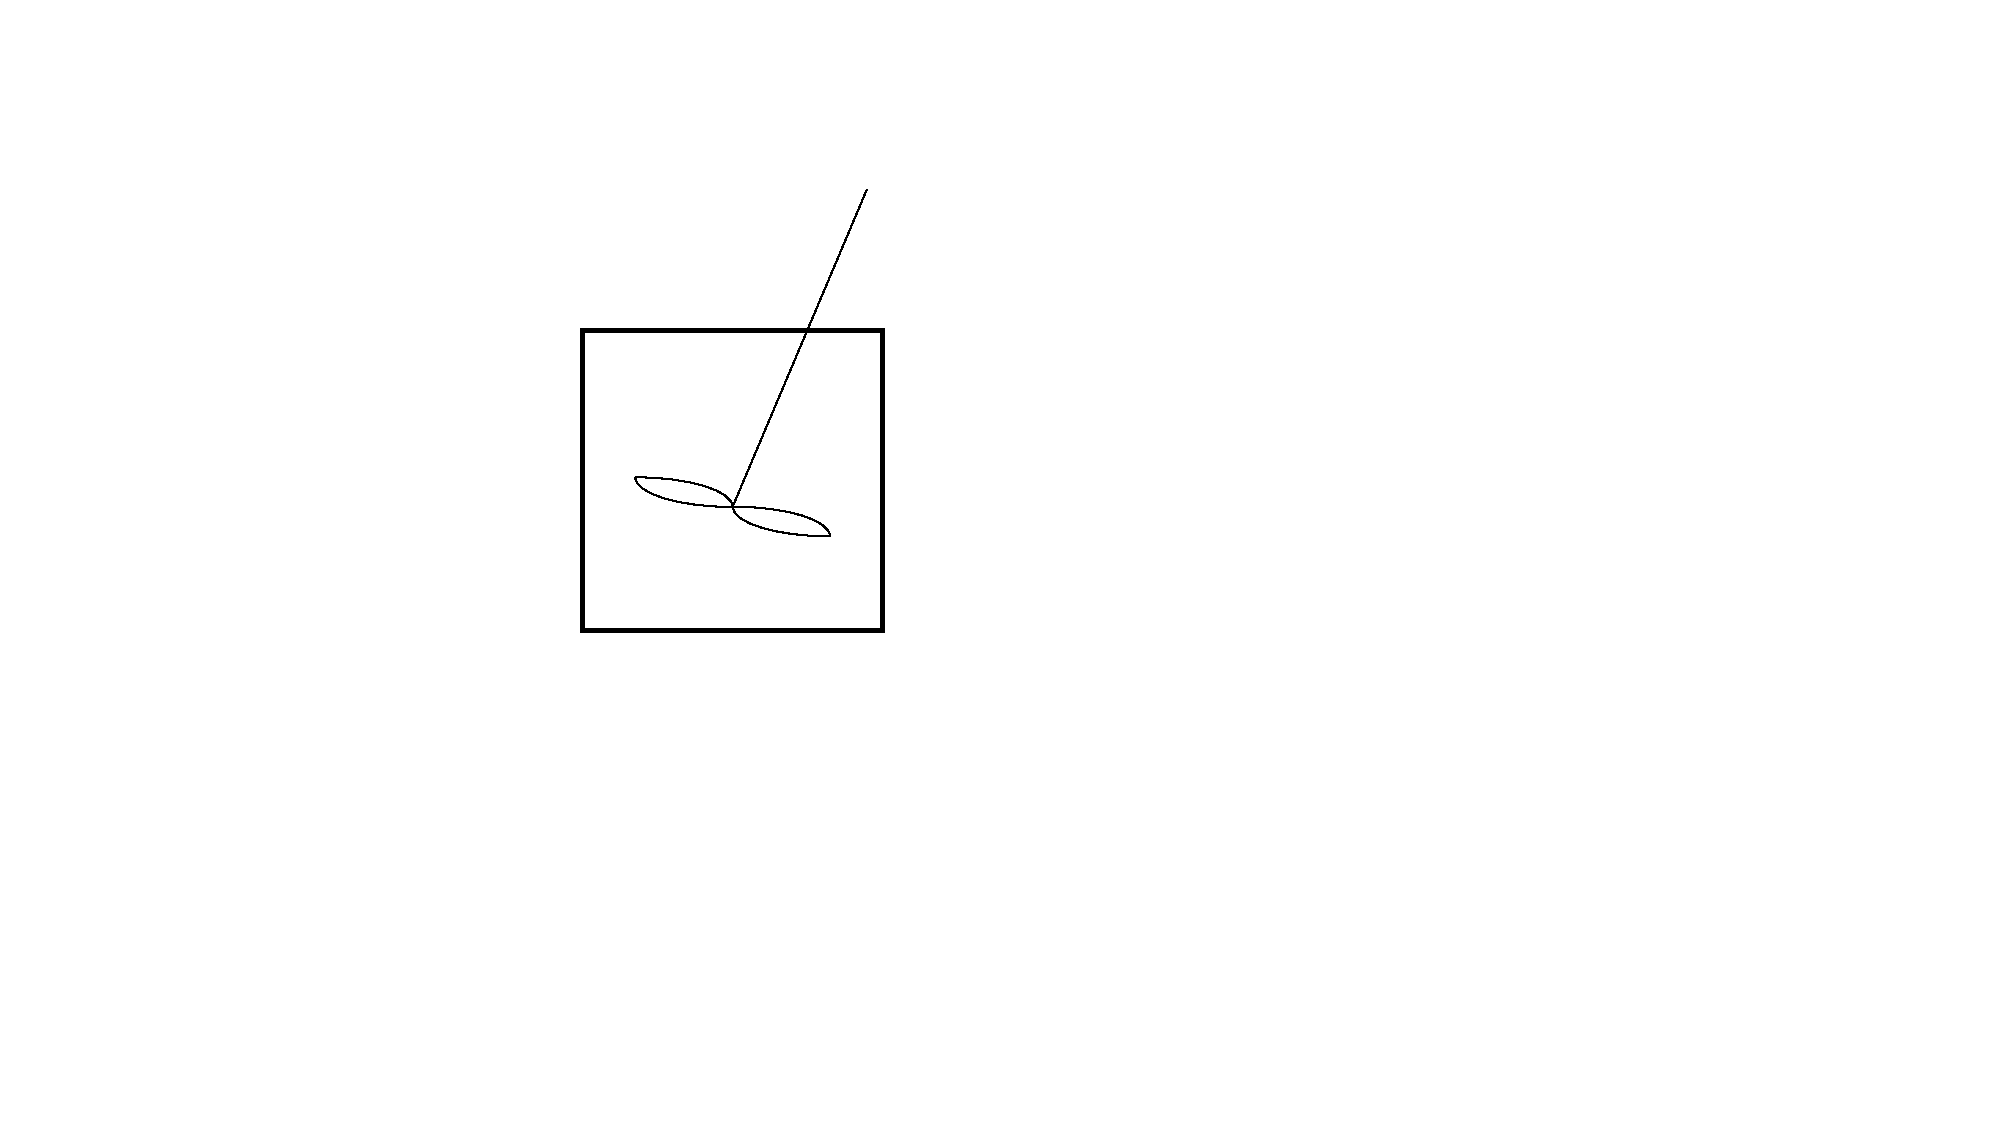
\includegraphics[width=0.3\linewidth]{../../.shared_files/reactor_fig}
\end{textblock*}
\vspace{1cm}
The ``Batch Aerobic Respiration'' scenario simulates the microbially mediated consumption of organic carbon with oxygen as the electron acceptor in a batch reactor over a week's time.

\EQ
\oxygen + \organiccarbon \rightarrow \carbondioxide + \water
\EN

\begin{itemize}
  \item Problem domain: 1 m$^3$
  \item Total simulation time: 1 week
  \item Maximum time step size: 1 hour
\end{itemize}

\end{frame}

%-----------------------------------------------------------------------------
\frame{\frametitle{Governing Reactive Transport Equations}

\large

\BA
  \frac{d \ci{i}}{d t} &\eq \nu_i I_r \\
  \frac{d X}{d t} &\eq yield_{X_{im}} I_r - k_\text{decay} \Xim \\
	I_r &\eq k_\text{max} X_{im} \frac{\ci{\oxygen}}{K_{\oxygen} + \ci{\oxygen}}\times\frac{\ci{\organiccarbon}}{K_{\organiccarbon} + \ci{\organiccarbon}}
\EA

%\bigskip
%\normalsize
\footnotesize
\begin{align*}
\ci{i} &\eq \text{aqueous concentration for species } i \\
\Xim &\eq \text{biomass concentration} \\
\nu_i &\eq \text{stoichiometry of species } i \text{ in reaction} \\
I_r &\eq \text{reaction rate} \\
yield_\Xim &\eq \text{yield or fraction of mass synthesized to biomass} \\
k_\text{decay} &\eq \text{first order decay rate} \\
k_\text{max} &\eq \text{maximum utilization rate} \\
K_{A_{aq}} &\eq \text{half saturation constant for species } A_{aq} \\
I_{C_{aq}} &\eq \text{inhibition factor for species } C_{aq}
\end{align*}

}

%-----------------------------------------------------------------------------
\section{Description of Input Deck}

%-----------------------------------------------------------------------------
\begin{frame}[fragile]\frametitle{SIMULATION}

\begin{itemize}
  \item Specify subsurface simulation
  \item Specify the use of the transport process model
\end{itemize}


\begin{semiverbatim}

SIMULATION
  SIMULATION_TYPE SUBSURFACE
  PROCESS_MODELS
    SUBSURFACE_TRANSPORT transport
      MODE GIRT
    /
  /
END

SUBSURFACE
  ...
END_SUBSURFACE
\end{semiverbatim}

\end{frame}

%-----------------------------------------------------------------------------
\begin{frame}[fragile]\frametitle{NUMERICAL\_METHODS}

\begin{itemize}
\item Due to the small problem size, request a direct solver instead of the default iterative BiCGStab Krylov solver.
\end{itemize}

\begin{semiverbatim}

NUMERICAL_METHODS TRANSPORT
  LINEAR_SOLVER
    SOLVER DIRECT
  /
END

\end{semiverbatim}

\end{frame}

%-----------------------------------------------------------------------------
\begin{frame}[fragile,containsverbatim]\frametitle{GRID}

\begin{itemize}
  \item Problem domain: 1 m$^3$
\end{itemize}

\begin{semiverbatim}

GRID
  TYPE STRUCTURED
  NXYZ 1 1 1
  BOUNDS
    0. 0. 0.
    1. 1. 1.
  /
END
\end{semiverbatim}

\end{frame}

%-----------------------------------------------------------------------------
\begin{frame}[fragile,containsverbatim]\frametitle{Fluid Properties}

\begin{itemize}
  \item Specify a reference water density of 1000 kg\,m$^{-3}$ for simplicity
\end{itemize}

\begin{semiverbatim}




REFERENCE_LIQUID_DENSITY 1000.d0

\end{semiverbatim}

\end{frame}

%-----------------------------------------------------------------------------
\begin{frame}[fragile,containsverbatim,allowframebreaks]\frametitle{CHEMISTRY}

\begin{itemize}
  \item Specify a microbial reaction with three aqueous species ($\oxygen$, $\organiccarbon$, $\carbondioxide$) and biomass ($\biomass$) growth and decay
\end{itemize}

\begin{semiverbatim}

CHEMISTRY
  PRIMARY_SPECIES
    O2(aq)
    CH2O(aq)
    CO2(aq)
  /
  IMMOBILE_SPECIES
    Biomass
  /
\end{semiverbatim}
\newpage
\normalsize
\begin{semiverbatim}
  MICROBIAL_REACTION
    REACTION O2(aq) + CH2O(aq) <-> CO2(aq) + H2O
    RATE_CONSTANT 4.d-2
    MONOD
      SPECIES_NAME O2(aq)
      HALF_SATURATION_CONSTANT 2.d-4
    /
    MONOD
      SPECIES_NAME CH2O(aq)
      HALF_SATURATION_CONSTANT 1.25d-5
    /
    BIOMASS
      SPECIES_NAME Biomass
      YIELD 1.d-4
    /
  /
\end{semiverbatim}
\normalsize
\begin{semiverbatim}
  IMMOBILE_DECAY_REACTION
    SPECIES_NAME Biomass
    RATE_CONSTANT 1.d-6
  /
  DATABASE ./aerobic_respiration.dat
  LOG_FORMULATION
  ACTIVITY_COEFFICIENTS OFF
  OUTPUT
    FREE_ION
    ALL
  /
END
\end{semiverbatim}

\end{frame}


%-----------------------------------------------------------------------------
\begin{frame}[fragile]\frametitle{MATERIAL\_PROPERTY}

\begin{itemize}
  \item A simple batch reactor full of water
\end{itemize}

\begin{semiverbatim}


MATERIAL_PROPERTY soil1
  ID 1
  POROSITY 1.d0
END
\end{semiverbatim}

\end{frame}

%-----------------------------------------------------------------------------
\begin{frame}[fragile]\frametitle{REGION}

\begin{semiverbatim}

REGION all
  COORDINATES
    -1.d20 -1.d20 -1.d20
    1.d20 1.d20 1.d20
  /
END

REGION middle   \bluecomment{! for observation point}
  COORDINATE 0.5d0 0.5d0 0.5d0
END

\end{semiverbatim}

\end{frame}

%-----------------------------------------------------------------------------
\begin{frame}[fragile]\frametitle{OBSERVATION}

\begin{itemize}
  \item Specify an observation point within the reactor
\end{itemize}

\begin{semiverbatim}


OBSERVATION
  REGION middle
END

\end{semiverbatim}

\end{frame}

%-----------------------------------------------------------------------------
\begin{frame}[fragile]\frametitle{OUTPUT}

\begin{itemize}
\item Output the observation point at every time step
\item Set output time units to days
\end{itemize}


\begin{semiverbatim}

OUTPUT
  PERIODIC_OBSERVATION TIMESTEP 1
  TIME_UNITS d
END
\end{semiverbatim}

\end{frame}

%-----------------------------------------------------------------------------
\begin{frame}[fragile]\frametitle{TIME}

\begin{itemize}
\item Set final simulation time to 1 week
\item Set initial time step size to 1 h
\item Set maximum time step size to 1 h
\end{itemize}


\begin{semiverbatim}


TIME
  FINAL_TIME 1.d0 w
  INITIAL_TIMESTEP_SIZE 1.d0 h
  MAXIMUM_TIMESTEP_SIZE 1.d0 h
END
\end{semiverbatim}

\end{frame}

%-----------------------------------------------------------------------------
\begin{frame}[fragile]\frametitle{TRANSPORT\_CONDITION {\large with Embedded CONSTRAINT}}

\begin{itemize}
  \item Embed transport constraint within transport condition
\end{itemize}
\begin{semiverbatim}
TRANSPORT_CONDITION initial
  TYPE ZERO_GRADIENT
  \redcomment{CONSTRAINT initial
    CONCENTRATIONS # [mol/L]
      O2(aq)    1.5d-3   F
      CH2O(aq)  2.d-3    F
      CO2(aq)   1.d-10   F
    /
    IMMOBILE    # [mol/m^3 bulk]
      Biomass   1.d-4
    /
  /}
END
\end{semiverbatim}

\end{frame}

%-----------------------------------------------------------------------------
\begin{frame}[fragile]\frametitle{INITIAL\_CONDITION}

\begin{itemize}
\item Couple the transport condition with the region for the initial condition
\item No boundary conditions
\end{itemize}

\begin{semiverbatim}

INITIAL_CONDITION
  TRANSPORT_CONDITION initial
  REGION all
END

\end{semiverbatim}

\end{frame}

%-----------------------------------------------------------------------------
\begin{frame}[fragile]\frametitle{STRATA}

\begin{itemize}
\item Couple material property with the region to define batch reactor
\end{itemize}

\begin{semiverbatim}

STRATA
  REGION all
  MATERIAL soil1
END


\end{semiverbatim}

\end{frame}

%-----------------------------------------------------------------------------
\begin{frame}[fragile]\frametitle{Running PFLOTRAN}

\begin{semiverbatim}

> cd $PFLOTRAN_DIR/
> cd shortcourse/exercises/0D_aerobic_respiriation
> pflotran -input_prefix aerobic_respiriation
> python plot_aerobic_respiriation.py

\end{semiverbatim}

\end{frame}

%-----------------------------------------------------------------------------
\begin{frame}[fragile]\frametitle{Add Inhibition Due to Oxygen Depletion}

\begin{semiverbatim}
  MICROBIAL_REACTION
    ...
    MONOD
      SPECIES_NAME CH2O(aq)
      HALF_SATURATION_CONSTANT 1.25d-5
    /
    \redcomment{INHIBITION
      SPECIES_NAME O2(aq)
      TYPE SMOOTHSTEP
      SMOOTHSTEP_INTERVAL 1.d-3
      INHIBIT_BELOW_THRESHOLD
      THRESHOLD_CONCENTRATION 2.5d-4
    /}
    BIOMASS
      SPECIES_NAME Biomass
      YIELD 1.d-4
    /
  /
\end{semiverbatim}

\end{frame}

%-----------------------------------------------------------------------------
\begin{frame}[fragile]\frametitle{Running PFLOTRAN}

\begin{semiverbatim}

> cd $PFLOTRAN_DIR/
> cd shortcourse/exercises/0D_aerobic_respiriation
> pflotran -input_prefix inhibited_aerobic_respiriation
> python plot_inhibited_aerobic_respiration.py

\end{semiverbatim}

\end{frame}

\end{document}
